\chapter{Teaching \cm Cosmology to the Public}\label{Ch:Planet}
Cosmology using the \cm line of hydrogen is a relatively new concept in the world of astronomy. It relies on radio telescopes, which have only been in general use for $\sim 50$ years. Measurements of the \cm signal from our own Milky Way Galaxy and other nearby galaxies have been used to study the neutral hydrogen gas distribution around the galaxies. 

On cosmological scales, where the \cm signals are $10^4 - 10^6$ times smaller than the foregrounds, the field is still in its infancy. There are many telescopes seeking to measure the \cm signal at redshifts ($z>1$), but as of yet, there has not been a significant detection in any of these cosmological redshift bands. 


\section{Overview}
One of the National Science Foundation grants that supports the Peterson group (\textcolor{red}{Add NSF reference number here.}) included \$20,000 for the creation of a $5-10$ minute planetarium show entitled $''$The Hydrogen Sky$''$. As producer, I have been working with a team of animators and artists to develop this show. 

I recruited two animators from Carnegie Mellon University's Entertainment Technology Center masters program\footnote{http://www.etc.cmu.edu/}, Alexander Moser and Meng Zhand. I also worked with Tom Casey and Warren Casey from Home Run Pictures\footnote{http://www.hrpictures.com/}, a local Pittsburgh animation company which specializes in full-dome planetarium productions. Additional support was provided by the Carnegie Science Center's Buhl Planetarium\footnote{http://www.carnegiesciencecenter.org/planetarium/} and its staff, specifically Frank Mancuso and Dr. Brendan Mullan.

\section{Storyboard and Script}
In order to complete the show, the first thing that we had to develop was a storyboard with visual queues to help the animators start creating content. From this first attempt at a storyboard, we identified a few key components for the show:

\begin{itemize}
\item Zoom out from the night sky to emphasize the connection to what we see every day.
\item Show the large scale structure, then show gaps where we don't have data. This is meant to demonstrate the need for \cm maps.
\item Have a sequence showing the interactions between hydrogen atoms and \cm photons in a cloud of gas. Include both stimulated emission and absorption, as well as a discussion of atomic spin.
\item Show photons travelling from the hydrogen gas cloud to earth, being redshifted along the way. 
\item Have a sequence of photons interacting with the Green Bank Telescope and being collected in the computers to make maps.
\item Make maps of the data from the Green Bank Telescope Intensity Mapping project and show the difference between the foregrounds and \cm maps. 
\item Show that the Green Bank maps are a very small fraction of the overall sky.
\item Have some video of the Canadian Hydrogen Intensity Mapping Experiment (CHIME).
\item Show how CHIME collects much more of the sky in a single day (aka drift scanning). 
\item Figure out a good conclusion to capture all of the science that can be done with \cm maps. Emphasize that CHIME is still under development. 
\end{itemize}

Once we had a general storyboard, we began refining it and writing a script that matched the visual components and told a clear story for a general audience. We went through a number of iterations on the script, trying to find a balance in communicating the important information without making the story too complicated. 

\subsection{Final Script}

\textcolor{red}{Add full text of the final script here.}
\textcolor{red}{Add single image shots for each paragraph with the script.}


\section{On-site Filming}
One of the key components of this show was on-site filming at a couple of real radio telescopes, the Robert C. Byrd Green Bank Radio Telescope (GBT)\footnote{https://science.nrao.edu/facilities/gbt/} and the Canadian Hydrogen Intensity Mapping Experiment (CHIME)\footnote{http://chime.phas.ubc.ca/}. For filming, we focused on still images and time lapses rather than video footage. Video footage did not translate well into the dome environment, as any irregular motion in the videos was magnified by the shape of the dome.  

We used two Nikon DSLR cameras (an old D80 and a new D800), with a rectangular lens on the D80 and a circular fisheye lens on the D800. The D80 was used primarily to capture images for creating panoramas of the locations we visited, while the fisheye was used for capturing single images and doing time-lapse videos. 

\begin{figure}[htb]
\centering
\begin{minipage}[b]{0.39\textwidth}
\centering
\includegraphics[width=0.95\linewidth]{Planetarium/figures/Filming_at_GBT_obs_deck.jpg}
\caption{Alex and Meng checking an image during filming.}
\label{Fig:GBT_obs_deck_film}
\end{minipage}%
\begin{minipage}[b]{0.02\textwidth}
\hspace{1cm}
\end{minipage}%
\begin{minipage}[b]{0.55\textwidth}
\centering
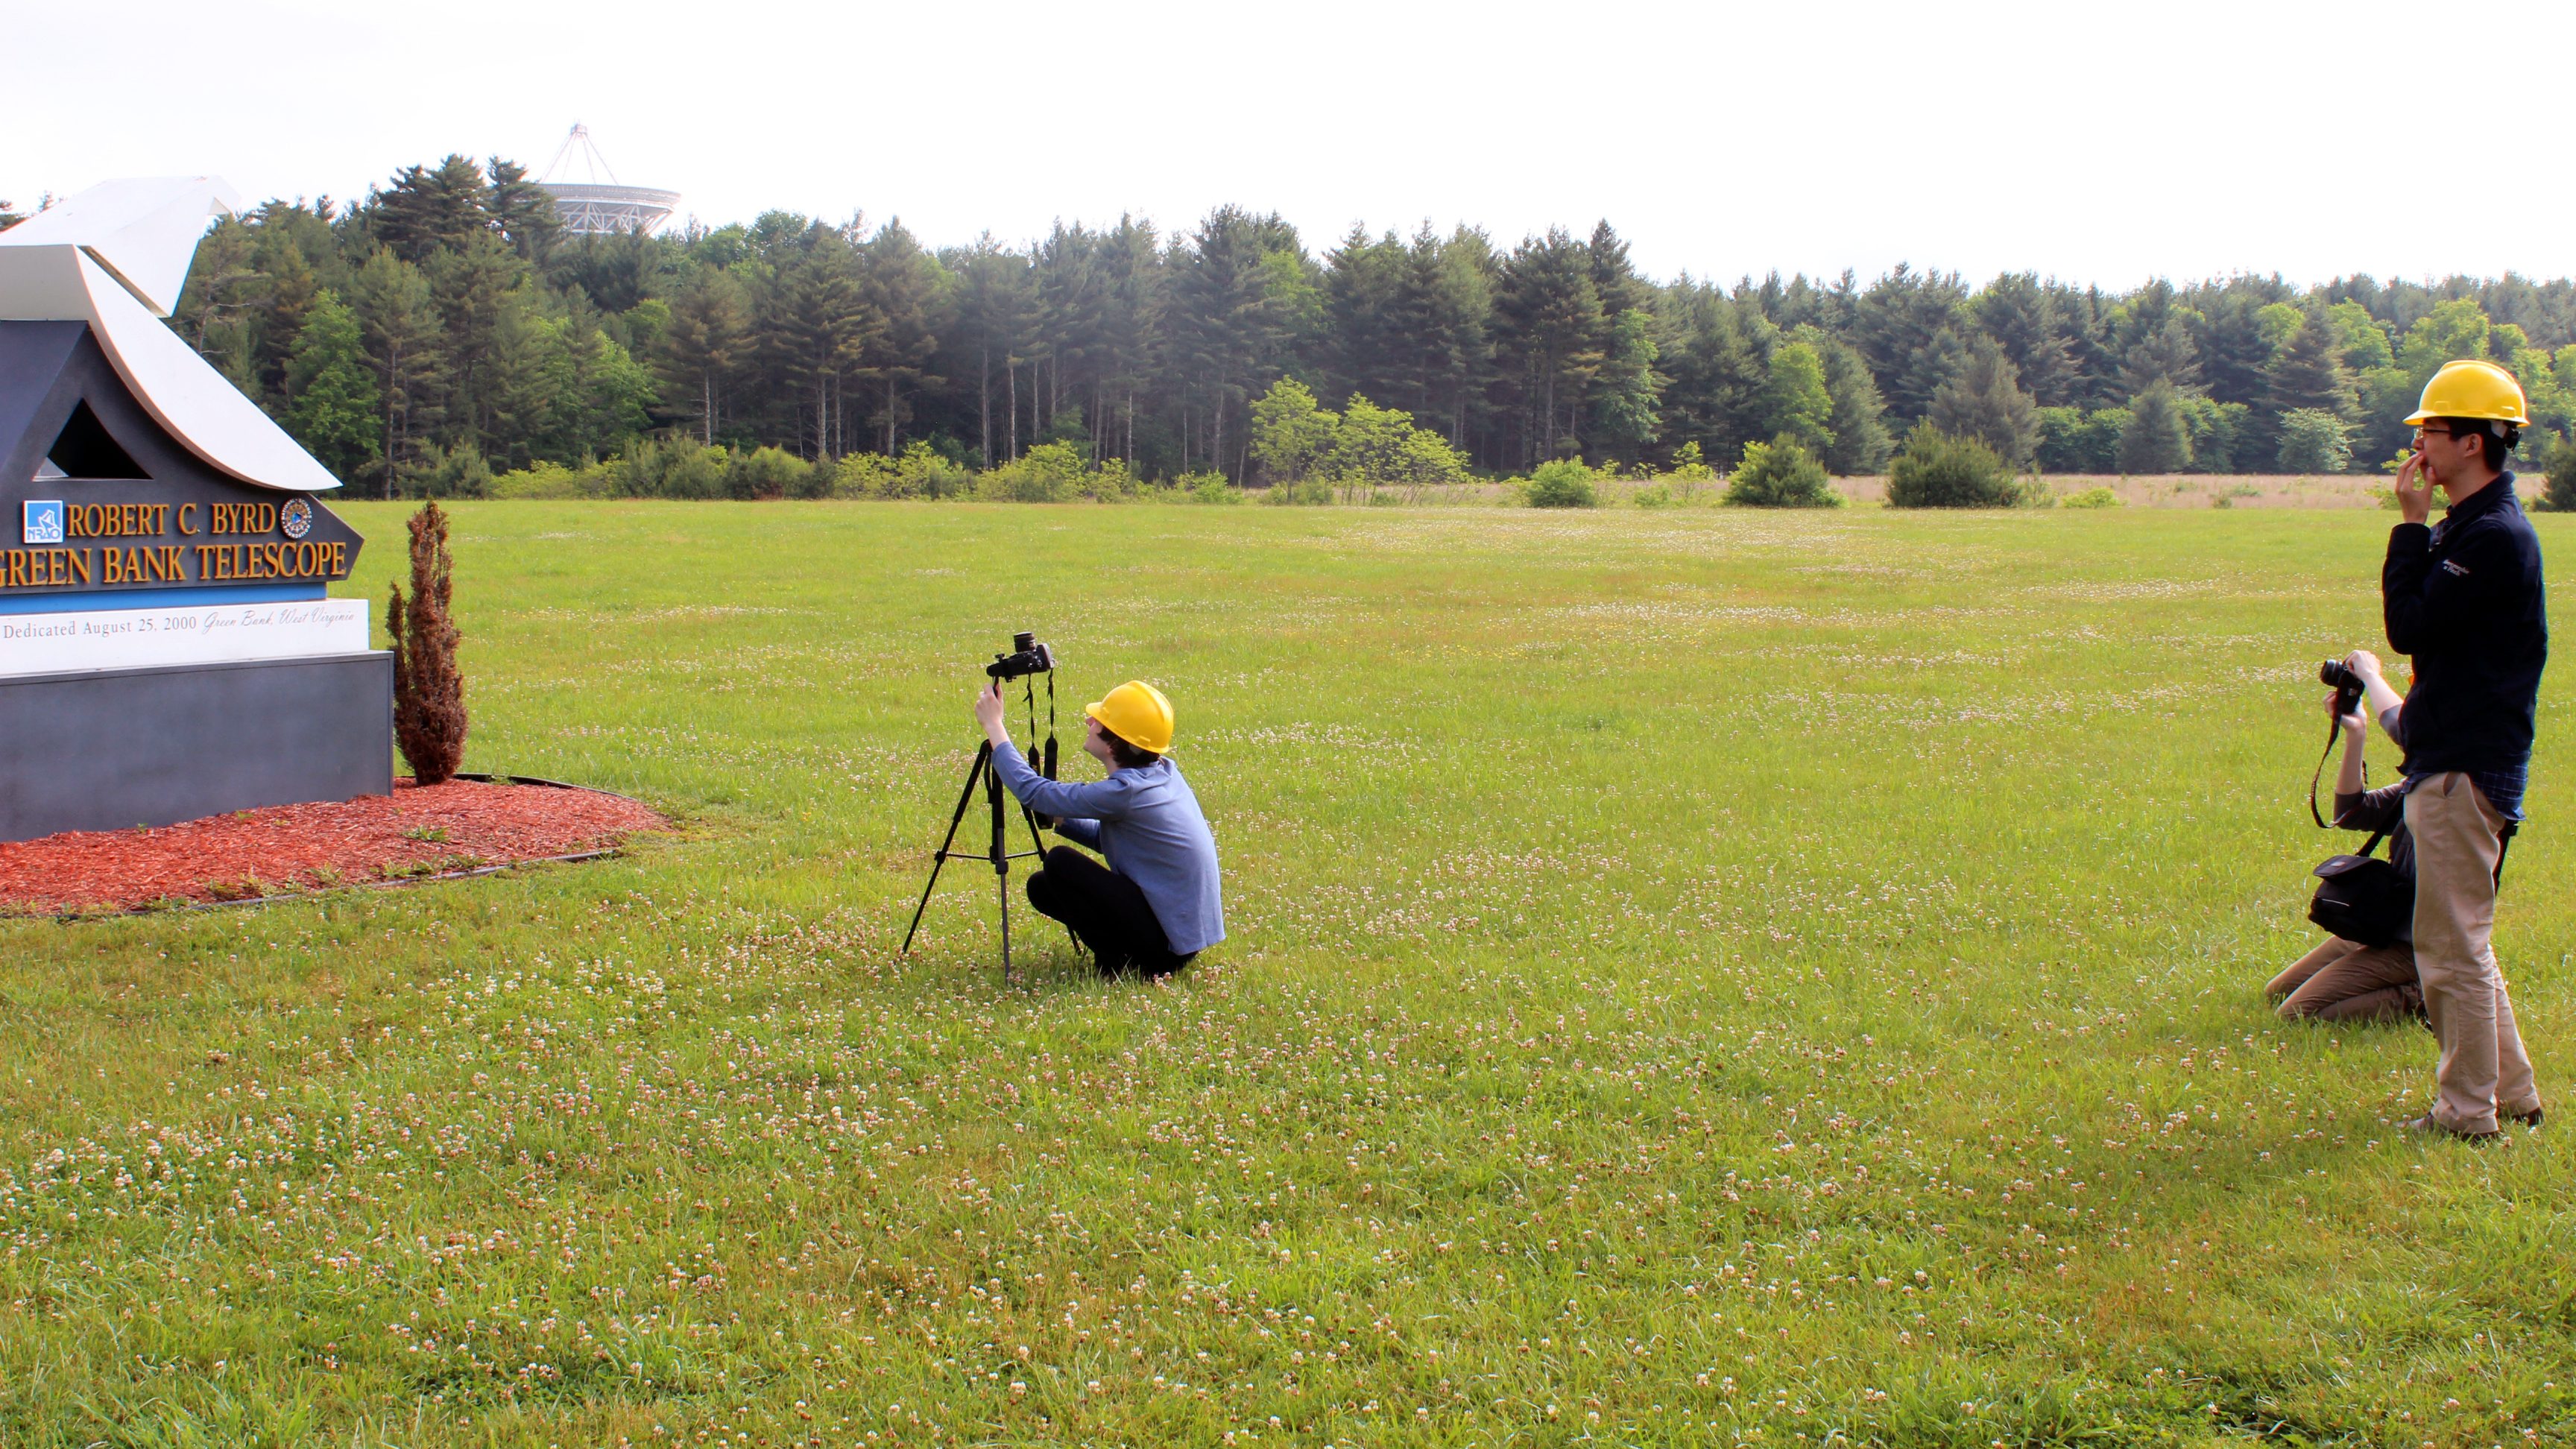
\includegraphics[width=0.95\linewidth]{Planetarium/figures/Filming_at_GBT_telescope_base.jpg}
\caption{Alex, Meng and Hsiu-Hsien taking multiple shots of the Green Bank Telescope from its base.}
\label{Fig:GBT_base_film}
\end{minipage}
\end{figure}

\begin{figure}[htb]
\centering
\begin{minipage}[b]{0.51\textwidth}
\centering
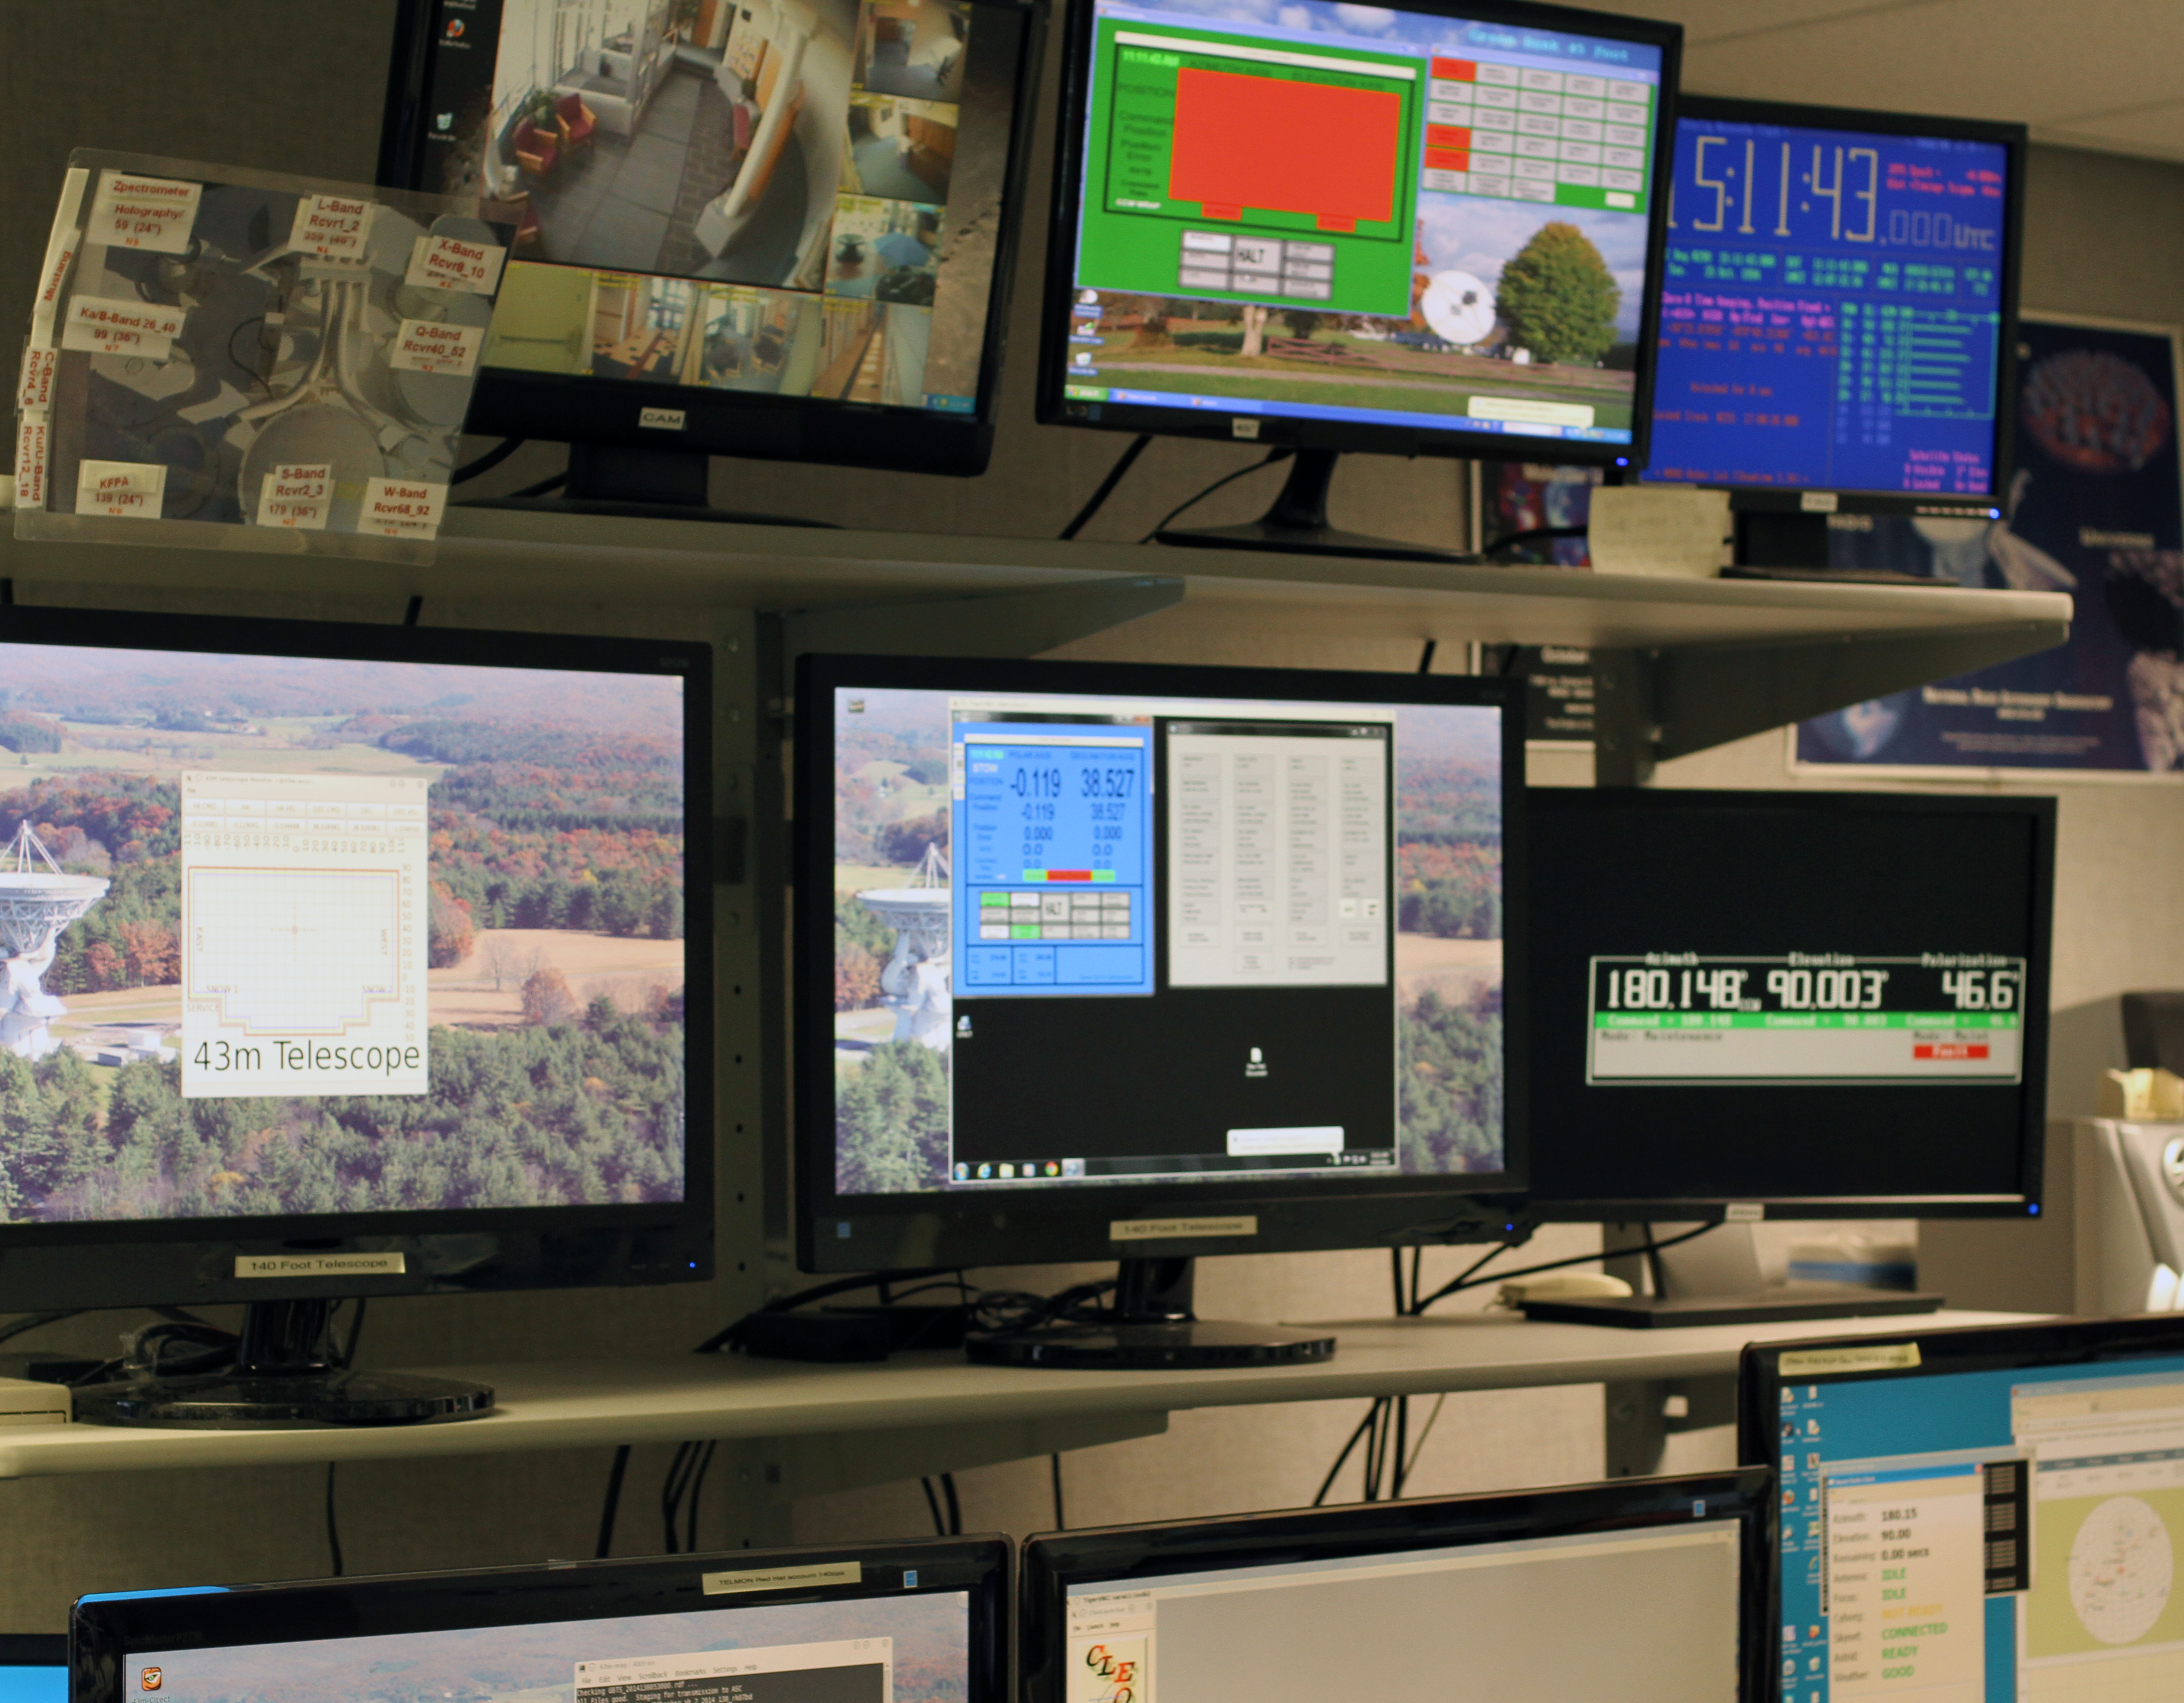
\includegraphics[width=0.95\linewidth]{Planetarium/figures/GBT_control_room.jpg}
\caption{Some of the monitors in the GBT control room, captured with the rectangular lens. }
\label{Fig:GBT_control}
\end{minipage}%
\begin{minipage}[b]{0.02\textwidth}
\hspace{1cm}
\end{minipage}%
\begin{minipage}[b]{0.43\textwidth}
\centering
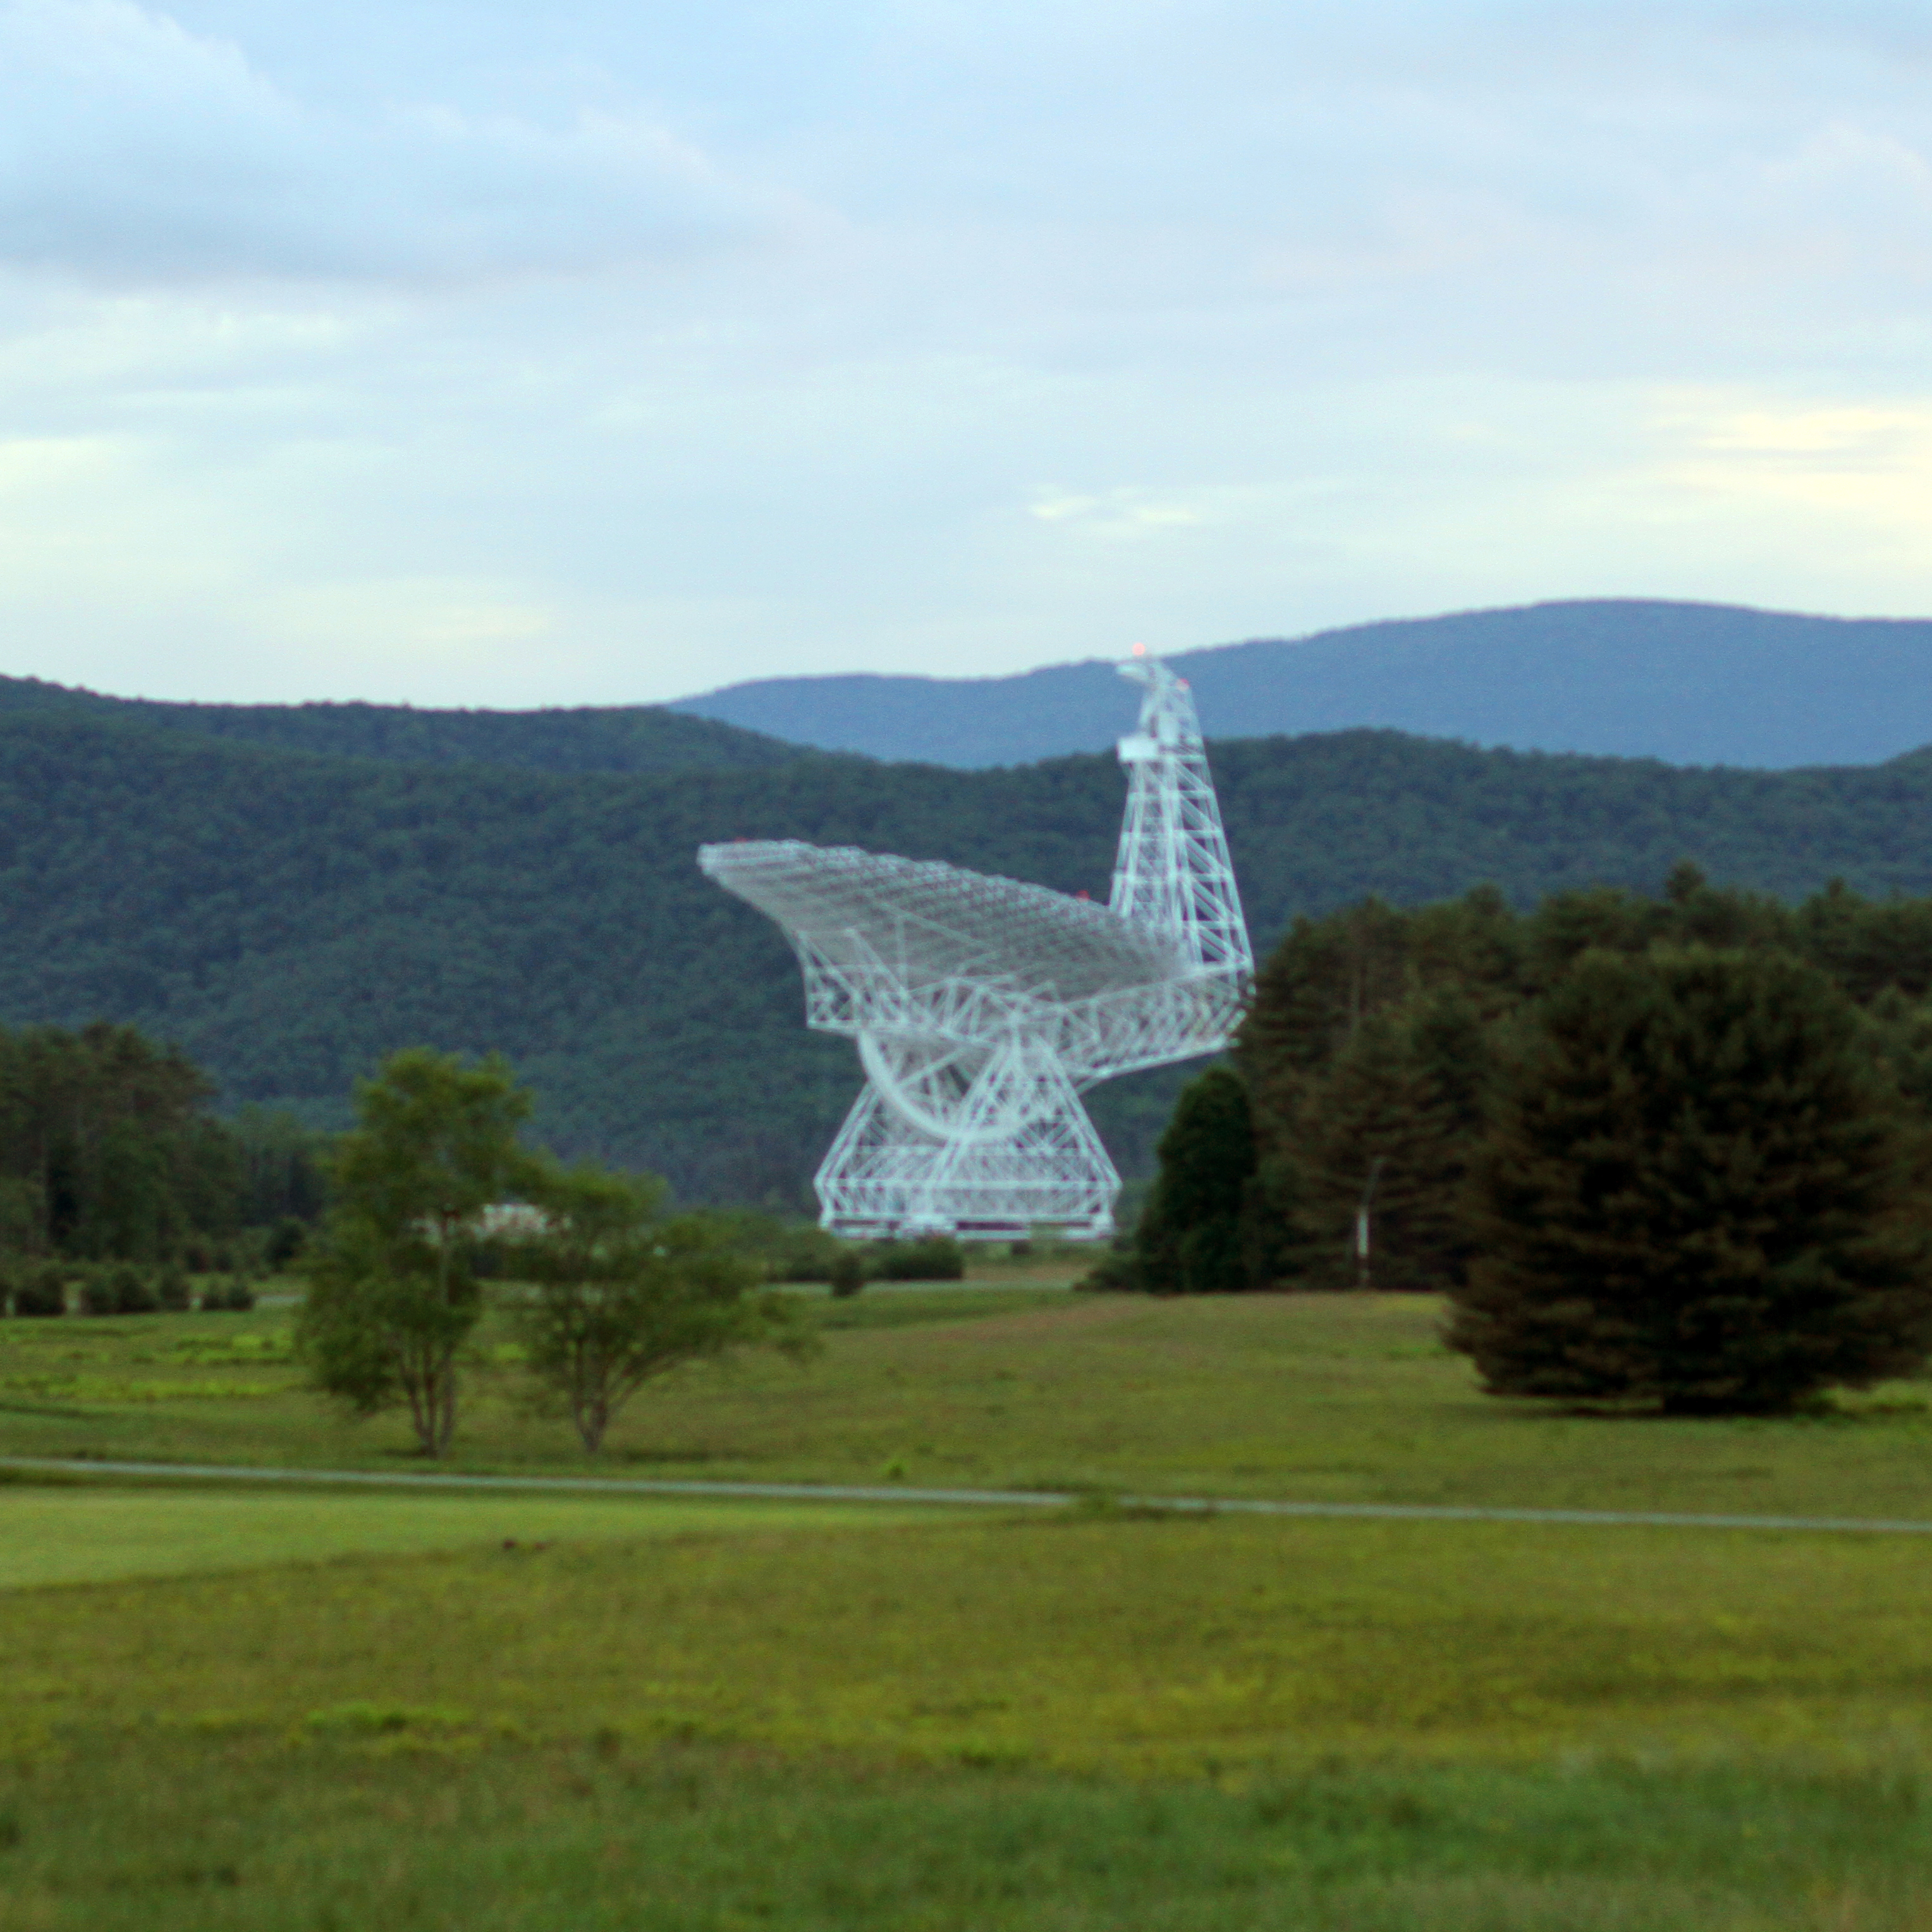
\includegraphics[width=0.95\linewidth]{Planetarium/figures/GBT_dusk.jpg}
\caption{Green Bank Telescope as seen from the observation deck, captured with the rectangular lens.}
\label{Fig:GBT_dusk}
\end{minipage}
\end{figure}

\begin{figure}[htb]
%\begin{center}
\centering
\begin{minipage}[b]{0.51\textwidth}
\centering
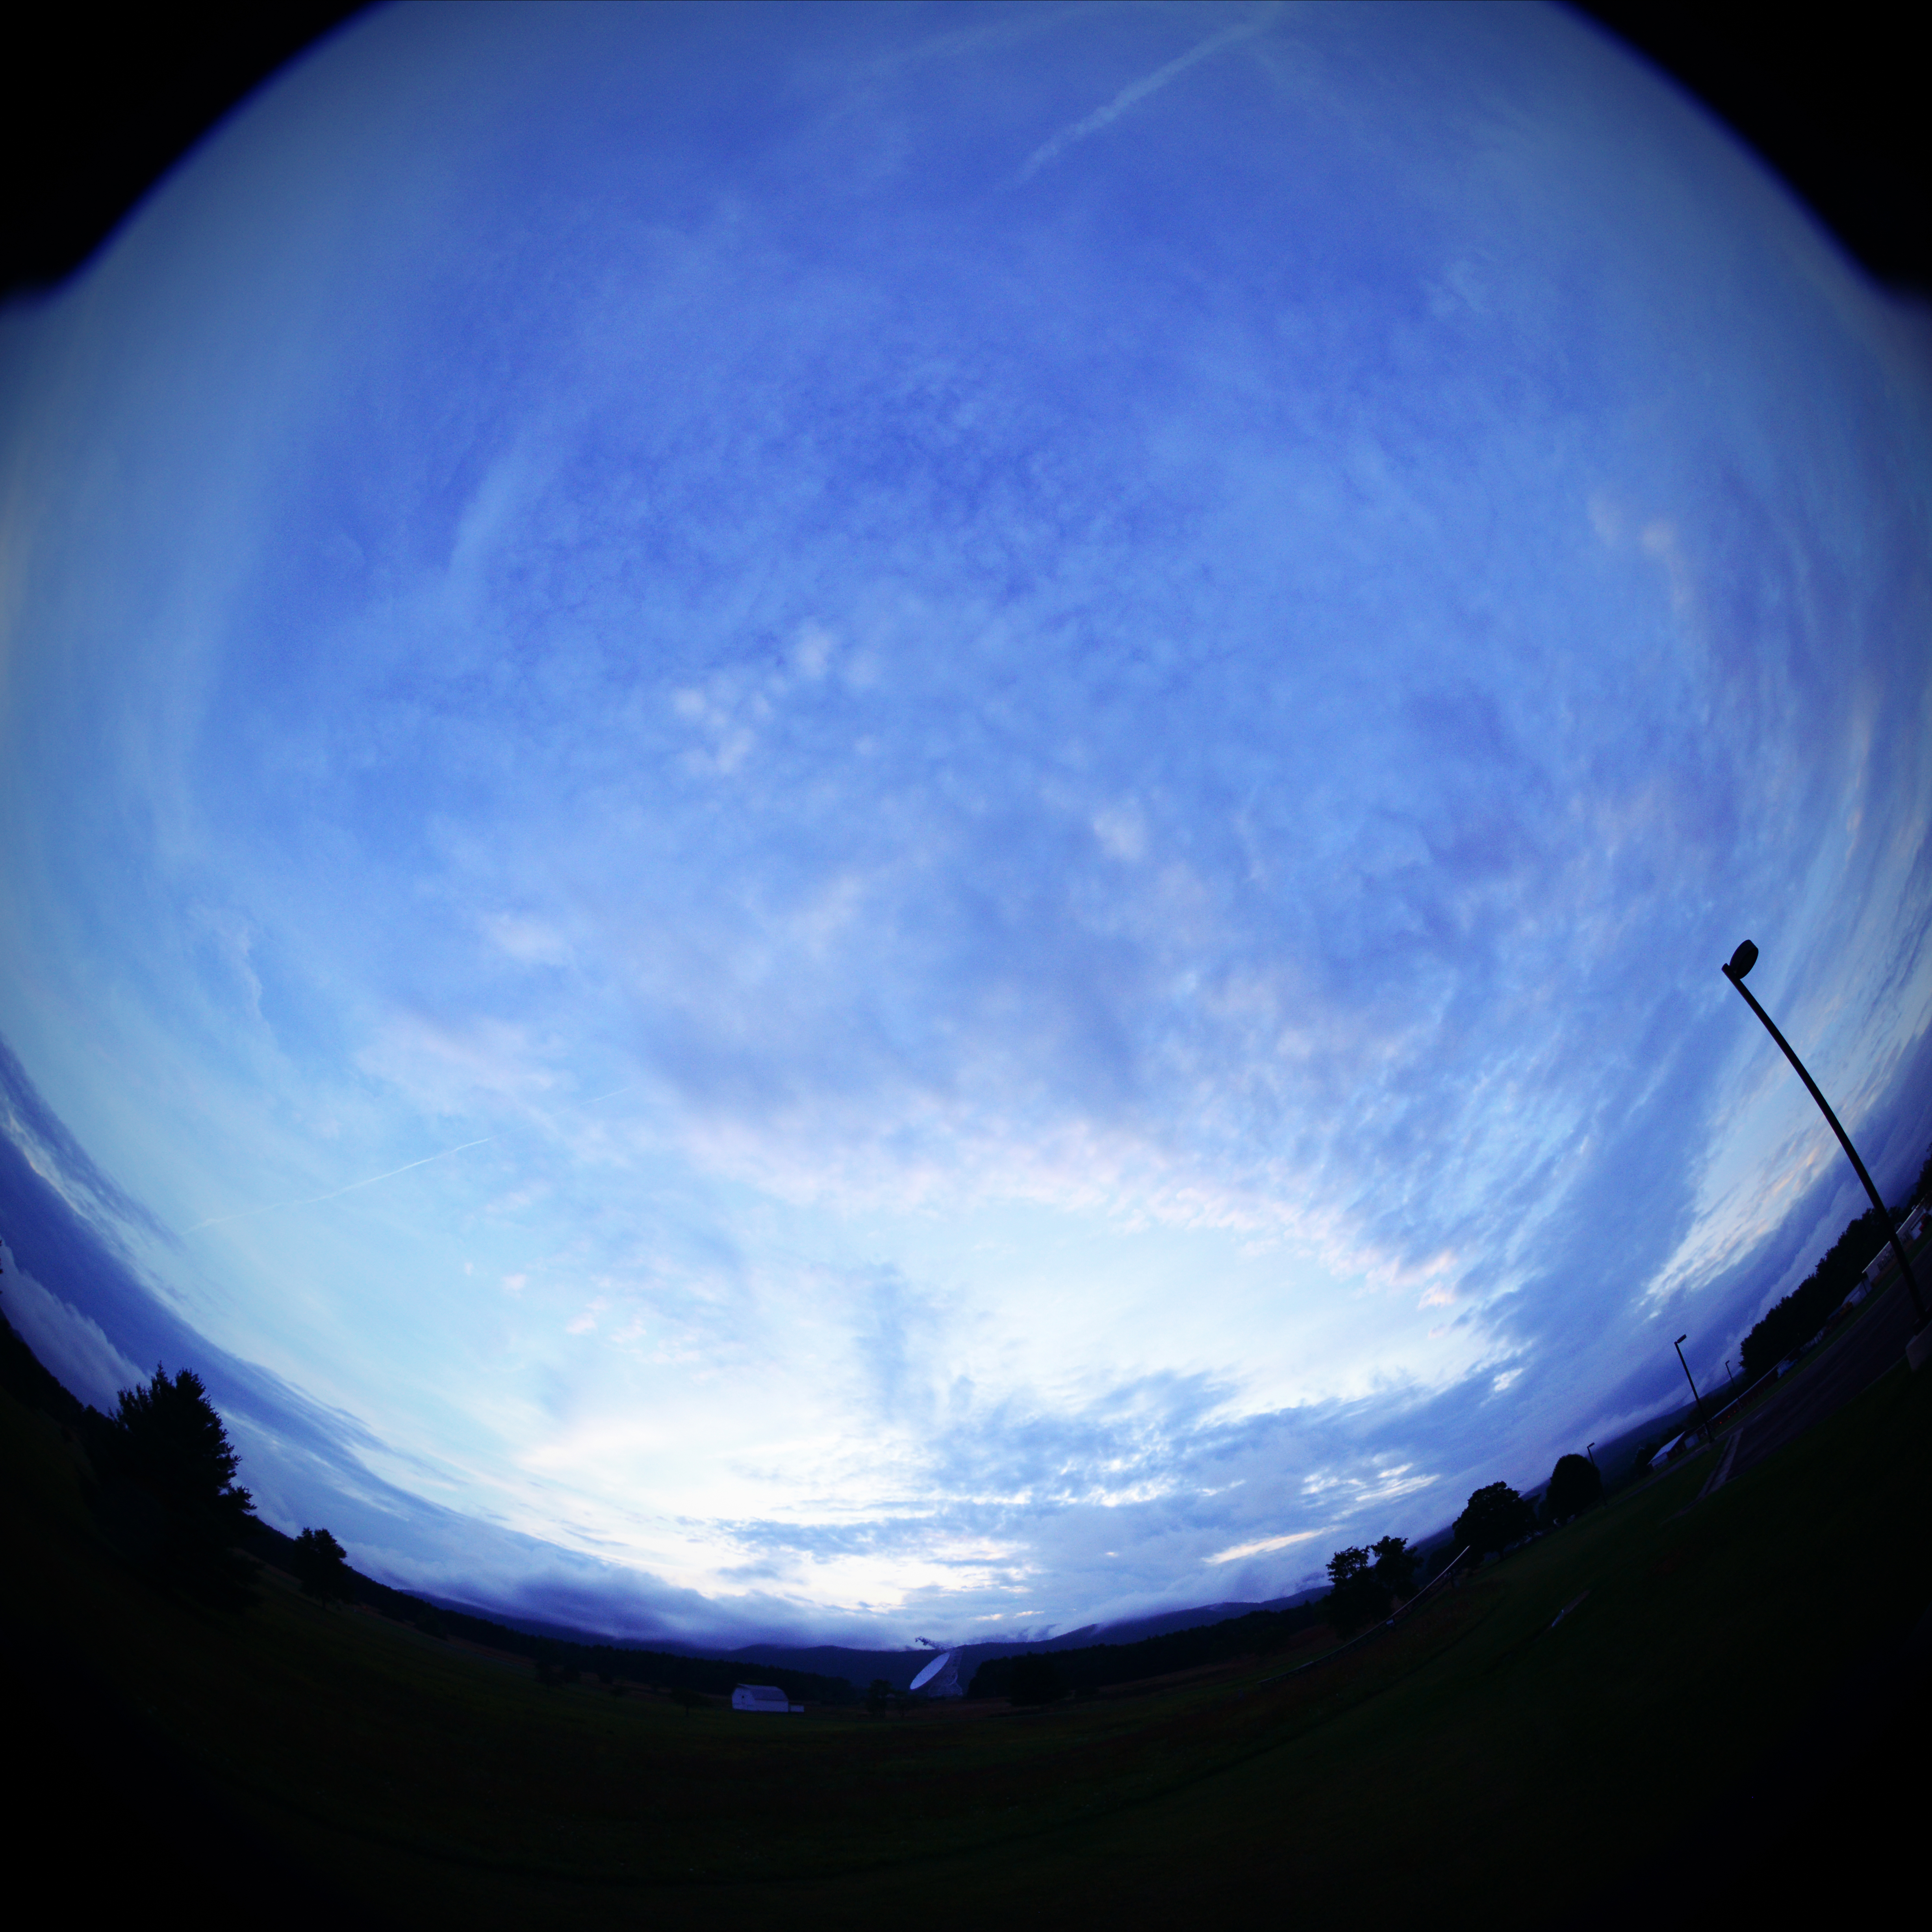
\includegraphics[width=0.95\linewidth]{Planetarium/figures/GBT_dusk_fisheye.jpg}
\caption{Green Bank Telescope as seen from the observation deck, captured with the fisheye lens.}
\label{Fig:GBT_dusk_fisheye}
\end{minipage}%
\begin{minipage}[b]{0.02\textwidth}
\hspace{1cm}
\end{minipage}%
\begin{minipage}[b]{0.43\textwidth}
\centering
%\end{center}
%\end{figure}
%\begin{figure}[htb]
%\begin{center}
\includegraphics[width=0.95\linewidth]{Planetarium/figures/GBT_base_render.jpg}
\caption{Green Bank Telescope as seen from its base, composited from images with the fisheye lens.}
\label{Fig:GBT_base_fisheye}
%\end{center}
\end{minipage}
\end{figure}

\subsection{Green Bank, WV}
We visited the National Radio Astronomy Observatory (NRAO) Green Bank site twice to gather footage in June and August 2014. We were able to stay on-site at the telescope and get footage both from the general site and from up close to the main 100 meter Green Bank Telescope. Footage had to be collected during the telescope maintenance time, as the cameras could be a source of Radio Frequency Interference (RFI) for the telescope when it was actually running.

Mike Holstine, the business manager at the Green Bank site, was our primary contact for the trips. He was able to get us a tour of the Robert C. Byrd Green Bank Radio Telescope, including taking two elevators up to the reciever on top of the telescope. Figures \ref{Fig:GBT_obs_deck_film} and \ref{Fig:GBT_base_film} show us filming at the GBT, while Figures \ref{Fig:GBT_control}, \ref{Fig:GBT_dusk}, \ref{Fig:GBT_dusk_fisheye}, and \ref{Fig:GBT_base_fisheye} show some of the images we were able to capture at the site with both the rectangular and fisheye lenses. 


\begin{figure}[htb]
\centering
\begin{minipage}[b]{0.57\textwidth}
\centering
\includegraphics[width=0.95\linewidth]{Planetarium/figures/Filming_at_CHIME.jpg}
\caption{Tabitha on top of one of the CHIME cylinders during filming. }
\label{Fig:CHIME_film}
\end{minipage}%
\begin{minipage}[b]{0.02\textwidth}
\hspace{1cm}
\end{minipage}%
\begin{minipage}[b]{0.37\textwidth}
\centering
\includegraphics[width=0.95\linewidth]{Planetarium/figures/CHIME_birdsnest.jpg}
\caption{Starlings hollowed out this nest in an RFI antenna on one of the CHIME cylinders.}
\label{Fig:CHIME_bird}
\end{minipage}
\end{figure}

\begin{figure}[htb]
\begin{center}
\includegraphics[width=0.95\linewidth]{Planetarium/figures/CHIME_cylinders.jpg}
\caption{CHIME pathfinder cylinders, captured with the rectangular lens. CHIME control room is inside the shipping container on the left side of the cylinders.}
\label{Fig:CHIME_cyl}
\end{center}
\end{figure}

\begin{figure}[htb]
%\begin{center}
\centering
\begin{minipage}[b]{0.47\textwidth}
\centering
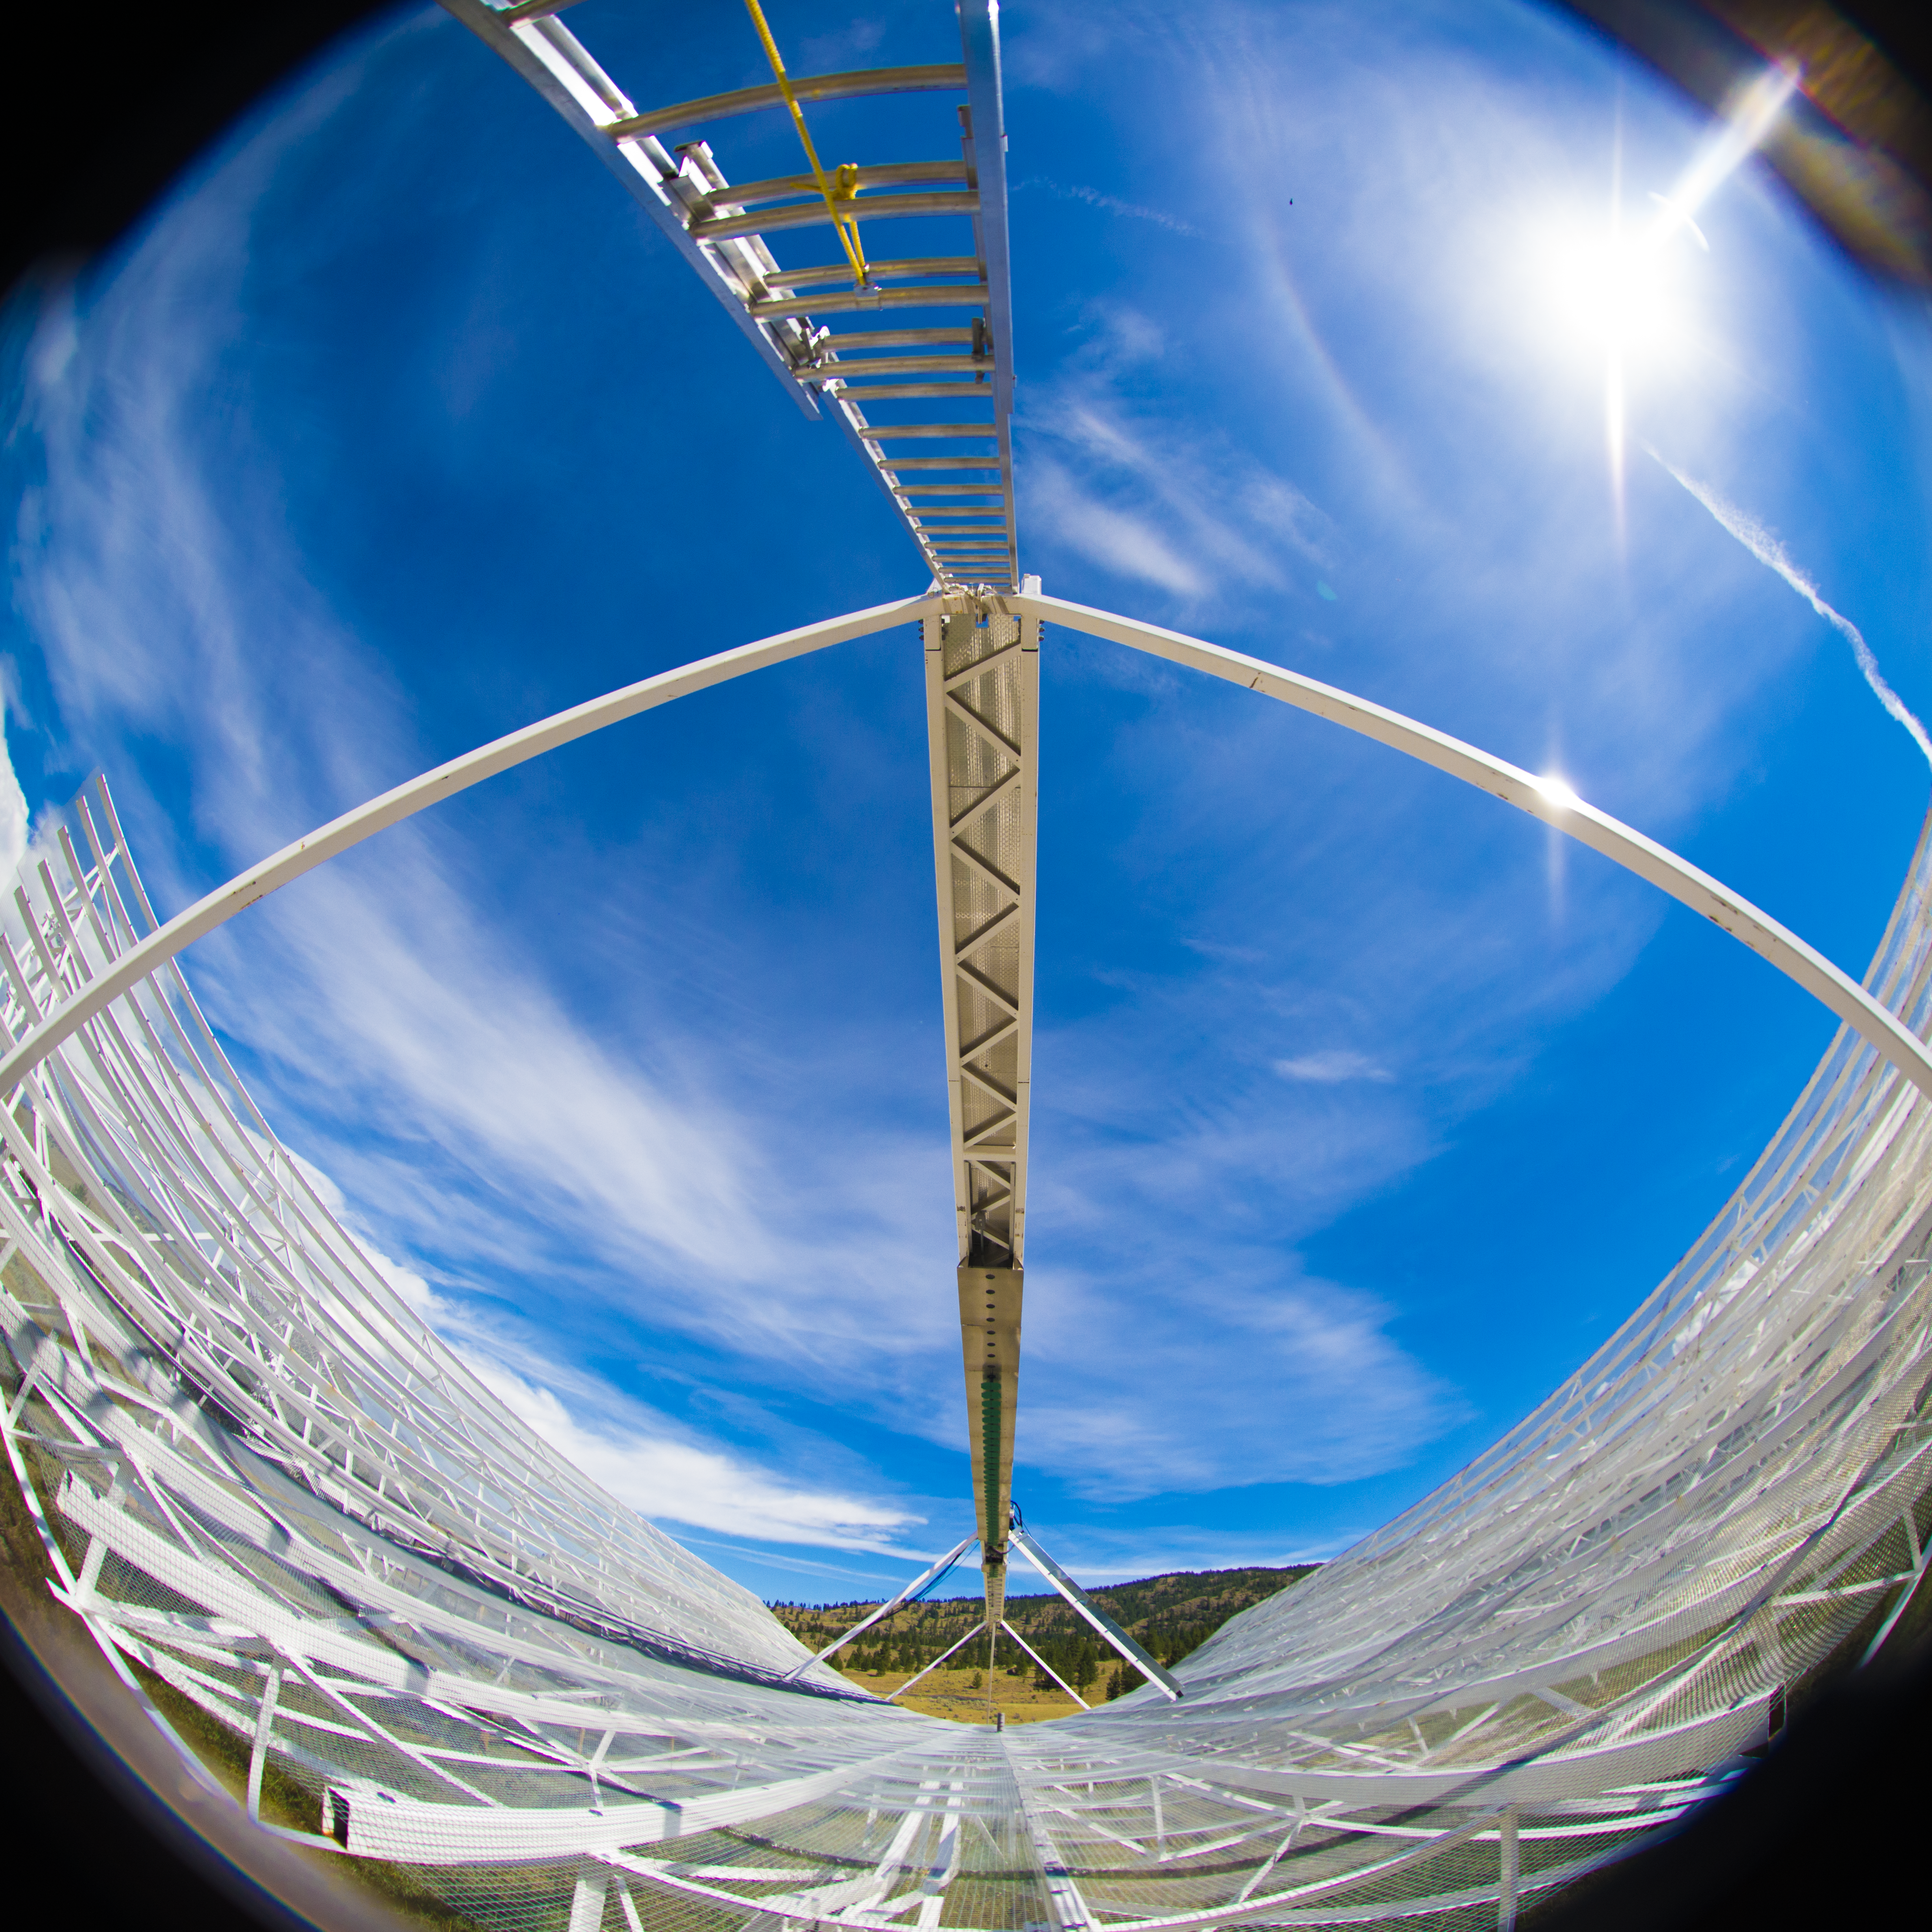
\includegraphics[width=0.95\linewidth]{Planetarium/figures/CHIME_cyl_fisheye.png}
\caption{Close up view of one of the CHIME cylinders, captured with the fisheye lens.}
\label{Fig:CHIME_cyl_fisheye}
%\end{center}
%\end{figure}
\end{minipage}%
\begin{minipage}[b]{0.02\textwidth}
\hspace{1cm}
\end{minipage}%
\begin{minipage}[b]{0.47\textwidth}
\centering
%\begin{figure}[htb]
%\begin{center}
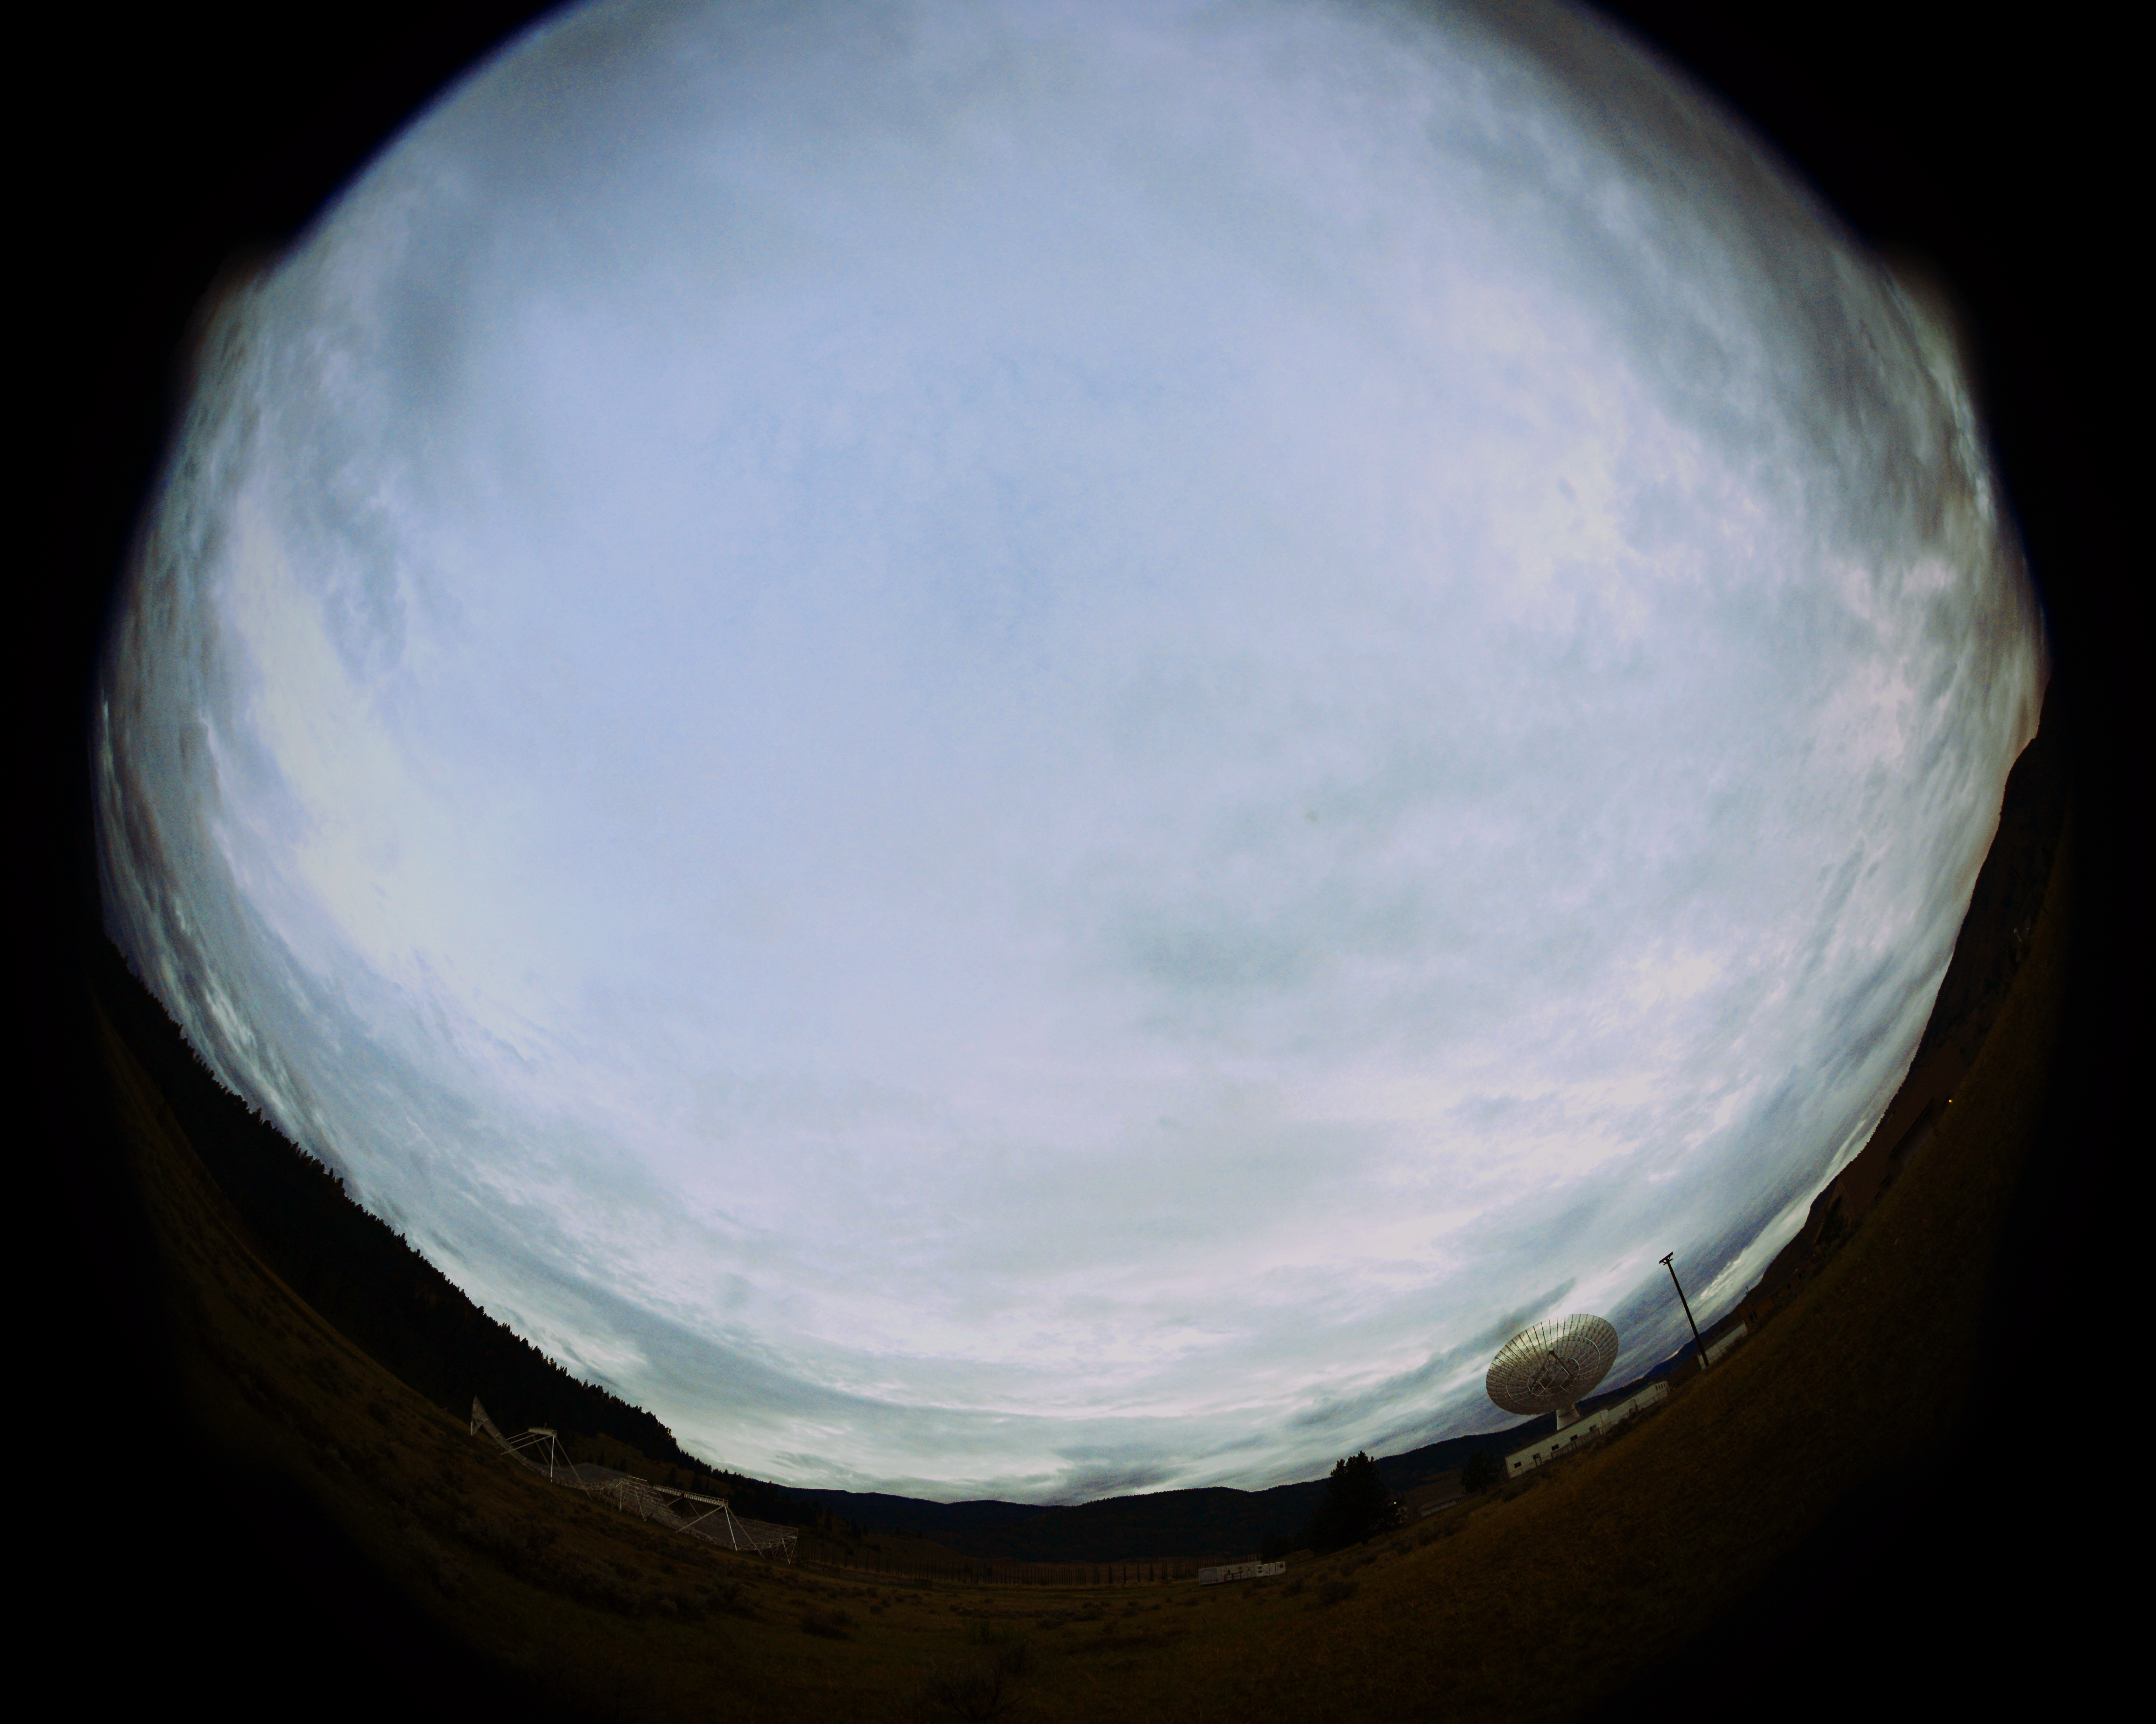
\includegraphics[width=0.95\linewidth]{Planetarium/figures/CHIME_dusk_fisheye.jpg}
\caption{CHIME cylinders at dusk along with the neighboring 26 m dish, captured with the fisheye lens.}
\label{Fig:CHIME_dusk_fisheye}
%\end{center}
\end{minipage}
\end{figure}

\subsection{Penticton, BC, Canada}
We visited the Dominion Radio Astrophysical Observatory (DRAO) site near Penticton in British Columbia, Canada where the CHIME telescope pathfinder is located and the full CHIME telescope will be built in June 2014. We stayed locally, in the city of Penticton, and were able to capture footage despite battling with rain for part of our visit. We were able to capture footage while the CHIME team was working on the computer system so that we didn't interfere with observations. 

Permission to film at the site was provided by Tom Landecker, the primary CHIME contact at the DRAO, as well as the rest of the CHIME team. David Hanna from McGill University was able to show us around the site and get us access during off hours so that we could film around dusk. Figure \ref{Fig:CHIME_film} shows us filming, while Figures \ref{Fig:CHIME_cyl}, \ref{Fig:CHIME_cyl_fisheye}, and \ref{Fig:CHIME_dusk_fisheye} show some of the images we were able to capture at the site with both the rectangular and fisheye lenses. 

\section{\cm Data Maps}


\section{Working in the Planetarium Environment}

\subsection{Technology}
\subsection{Visual Differences}

\section{Audio Production}

\subsection{Narration}
\subsection{Music and Sound Effects}

\section{Feedback and Evaluation}

